\section{Dual Learning Program Repair}



After the representation learning step, we obtain the vectorized AST
$T^{M}_b$ for the buggy method $M$ and the vectorized AST subtree
$T^{s}_b$ for the buggy statement $s$, as well as the one for the
respective fixed method $T^{M}_f$ and the one for the respective fixed
statement $T^{s}_f$. $T^{M}_b$ and $T^{M}_f$ are used at the input and
output layers of the context learning model (\code{CCL}); and
$T^{s}_b$ and $T^{s}_f$ are used at the input and output layers of the
transformation learning model (\code{CTL}). Let us explain the dual
learning framework for \code{CCL} and \code{CTL}.

%After having the $Tree_m$, $Tree_{mf}$ pair and $Tree_s$, $Tree_{sf}$ pair from the first step, \tool uses them as the input and the ground truth to train the dual learning program repair model in this step. \tool uses the generated after fixing AST $Tree'_m$ and after fixing subtree of AST $Tree'_s$ as output for this step when making the prediction. Specifically, there are two small steps, including the AST node representation learning and the dual learning framework.


\subsection{Cross-stitch Unit}

We perform a joint training between \code{CCL} and \code{CTL} via
cross-stitch units~\cite{misra2016cross}. Let us first explain the
cross-stitch unit and then how we leverage it for the auto bug-fixing
problem.

\begin{figure}[t]
	\centering
	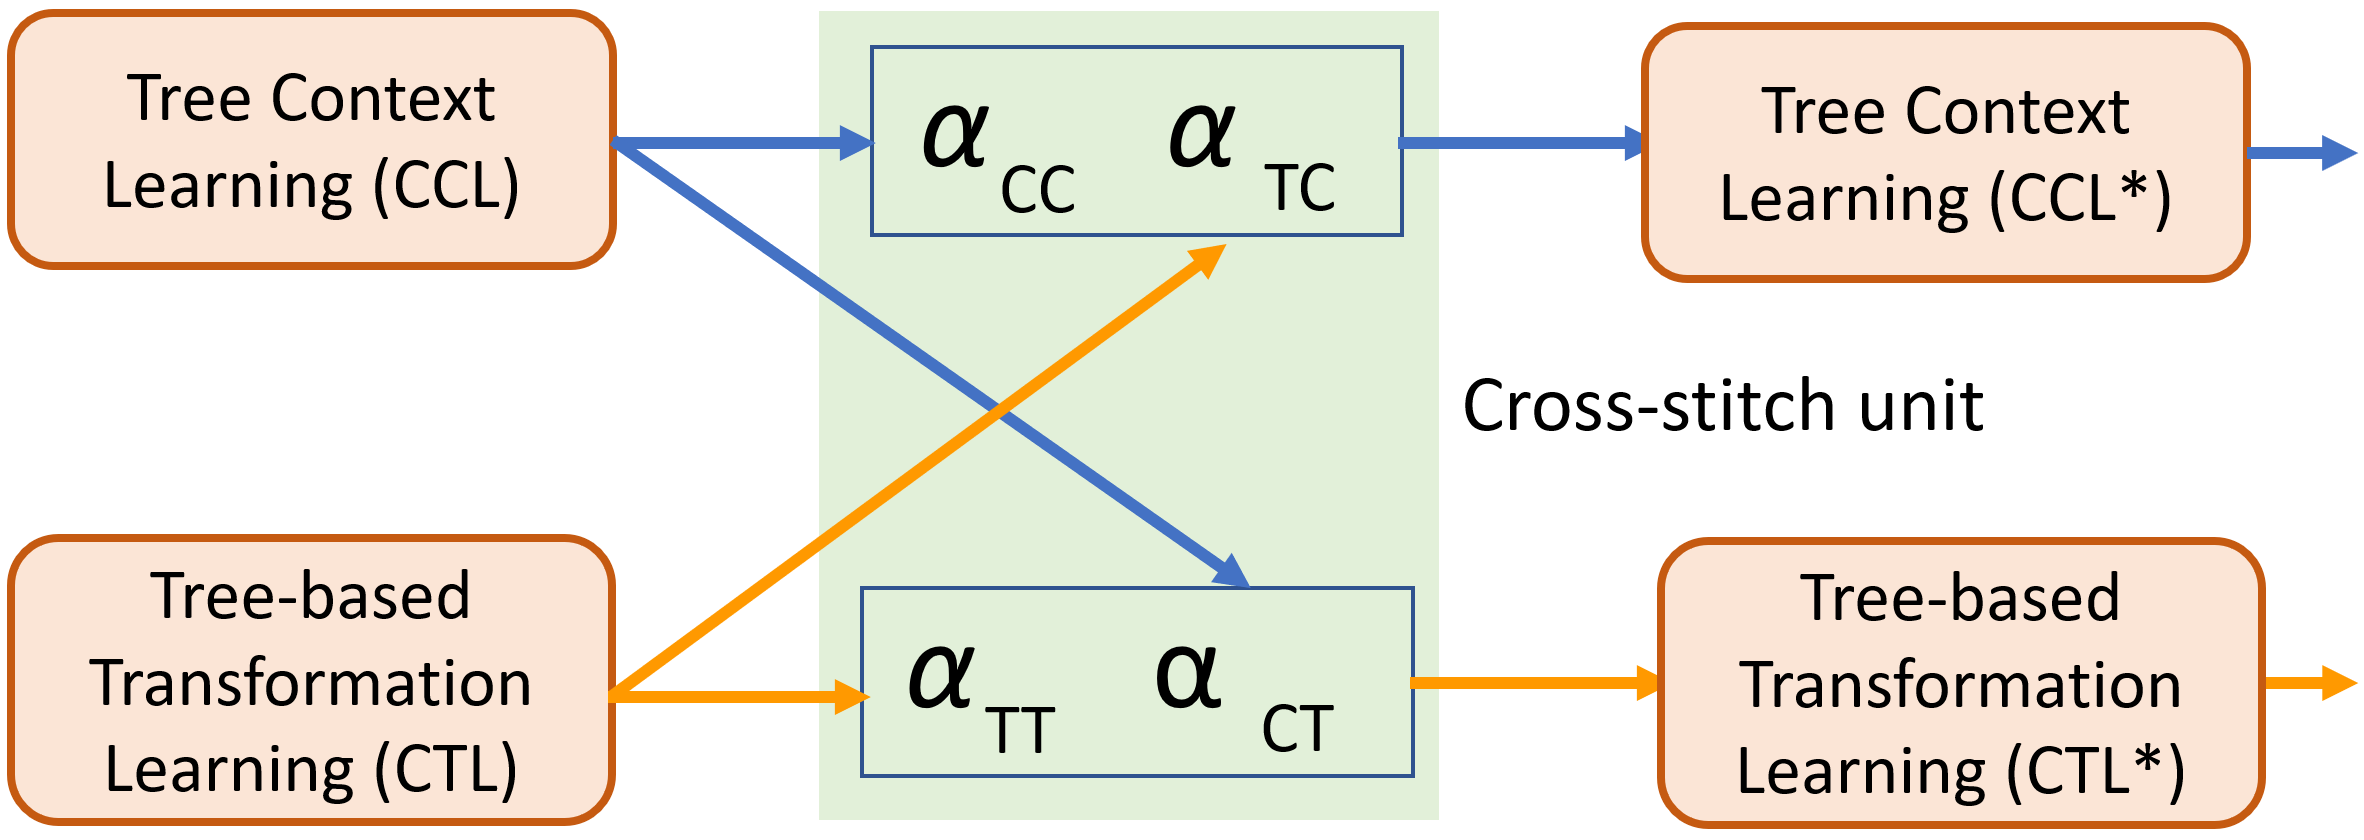
\includegraphics[width=3.2in]{graphs/cross-stitch}
	\caption{Cross-Stitch Unit for Joint Training~\cite{misra2016cross}}
	\label{fig:cross-stitch}
\end{figure}

In Figure~\ref{fig:cross-stitch}, to apply dual learning between
\code{CCL} and \code{CTL}, we use the cross-stitch unit to connect
them together. The sharing of representations between \code{CCL} and
\code{CTL} is modeled by the learning a linear combination of the
input features from the vectorized AST (sub)trees. The top sub-network
of the cross-stitch unit get direct supervision from \code{CCL} and
indirect supervision from \code{CTL}. Cross-stitch units help
regularize both \code{CCL} and \code{CTL} by learning and enforcing
shared representations by combining feature
maps~\cite{misra2016cross}.

The goal of cross-stitch unit is to learn such a linear combination of
both inputs from \code{CCL} and \code{CTL}, which is parameterized
using the weights $\alpha$. The output of the cross-stitch unit is
computed as:
\begin{equation}\label{eq:cross-stitch}
	\begin{bmatrix}
		I_C\\
		I_T
	\end{bmatrix}
	=
	\begin{bmatrix}
		\alpha_{CC} &  \alpha_{CT} \\
		\alpha_{TC} &  \alpha_{TT}
	\end{bmatrix}
	\begin{bmatrix}
		O_C\\
		O_T
	\end{bmatrix}
\end{equation}
$I_C$ and $I_T$ are the inputs for the cross-stitch unit, which are
the outputs from a layer of \code{CCL} and \code{CTL}. $O_C$ and $O_T$
are the outputs from the cross-stitch unit, which can be used as the
inputs for the next layer of the two models. In this case, the next
layers (noted as \code{CCL*} and \code{CTL*}) are the ones with the
shared representations and having the joint training. More details are
in~\cite{misra2016cross}.

\subsection{Dual Learning between CCL and CTL}

First, \tool uses two separate attention-based seq2seq frameworks to learn the code fixing for both the method-level and the statement-level. We all use the tree-based deep learning model to process the AST or subtree of AST for the encoder and decoder of these two tasks. Based on the recent study, we select a well-performed baseline TreeCaps \cite{bui2021treecaps} here to do so. Between the encoder and decoder, there is an attention layer for both tasks to help improve the accuracy of generating the fixing.

In the regular attention-based seq2seq model, the hidden status $H$ is directly passed to the attention layer. However, \tool uses a cross-stitch unit to accept the hidden status $H_m$ and $H_s$ from both method-level and the statement-level to achieve the dual learning. And then, the \tool passes the output of the cross-stitch unit to the method-level and statement-level attention layer. Just like the Figure \ref{program-repair} shown, the output from the encoder does not go to the attention layer. They go to the cross-stitch unit instead. The cross-stitch unit helps both the method-level and the statement-level attention-based seq2seq model catch the input features within the buggy method and the buggy statement.

\begin{figure}[t]
	\centering
	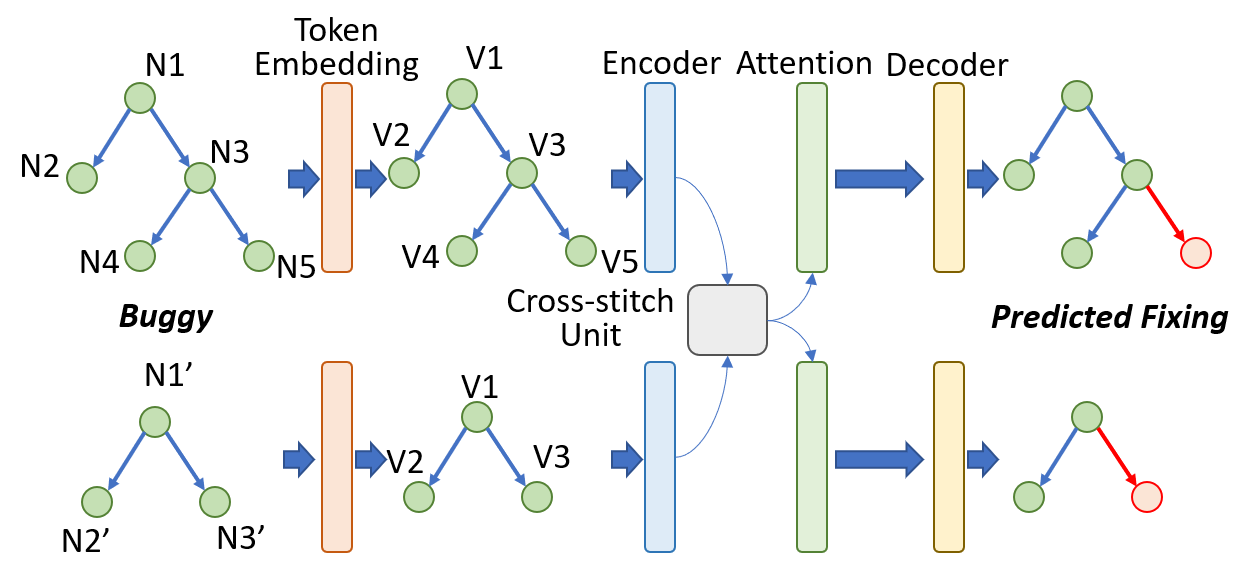
\includegraphics[width=3.2in]{graphs/program_repair.png}
	\caption{Dual Learning Program Repair}
	\label{program-repair}
\end{figure}

As for the TreeCaps model \tool is using, it is built on top of $k$ TBCNN layers \cite{mou2014tbcnn}. So, for the TBCNN layer $k$, the output of the convolution window is calculated as:

\begin{equation}\label{eq:1}
	Y = tanh(\sum_{i=1}^{N}[\Delta^t_iW^t + \Delta^t_iW^t + \Delta^t_iW^t]X_i + b)
\end{equation}

Where $\Delta$ are weights calculated corresponding to the depth and the position of the nodes. One can see this as a
way to learn the position of a node inside AST. $W$ is the trainable matrix; $b$ is the bias; $N$ is the total number of nodes in the convolution window. TreeCaps merges the output from all TBCNN layers by using a non-linear squash
function \cite{sabour2017dynamic}. For an AST node $j$, we calculate the capsules $u_j$ as:

\begin{equation}\label{eq:2}
	u_j = \frac{||c_j||^2}{||c_j||^2+1}\frac{c_j}{||c_j||}
\end{equation}

By merging all capsules as a list with the deep traversal order, \tool has the output $H$ for the TreeCaps model.

After \tool has $H_m$ and $H_s$ for both method-level and statement-level in the encoder, we aim to learn the linear combinations of both inputs of the cross-stitch unit. The output of the cross-stitch unit is computed as:

\begin{equation}\label{eq:3}
	\begin{bmatrix}
		X_m\\
		X_s
	\end{bmatrix}
	=
	\begin{bmatrix}
		\alpha_{mm} &  \alpha_{ms} \\
		\alpha_{sm} &  \alpha_{ss}
	\end{bmatrix}
	\begin{bmatrix}
		H_s\\
		H_m
	\end{bmatrix}
\end{equation}

Where $\aleph$ is the trainable weight matrix, $X_m$ and $X_s$ are the inputs for the attention layers of both two tasks. For $X_m$ and $X_s$, they both contain the information learned from the method-level and the statement-level, which achieves the main goal of the dual learning framework. From formula \ref{eq:3}, we could know:

\begin{equation}\label{eq:4}
	X_m = \alpha_{mm}H_m + \alpha_{ms}H_s
\end{equation}
\begin{equation}\label{eq:5}
	X_s = \alpha_{sm}H_m + \alpha_{ss}H_s
\end{equation}

However, if the $H_s$ and $H_m$ have different sizes, we need to resize them to be consistent. If the size needs to be increased, we use the bilinear interpolation for resizing. If the size needs to be reduced, we do the center crop on the matrix to match the required size.

After solving this, here is one last problem the dual learning may face. When making the prediction, because we don't know how the tree structure changes, \tool needs to have a size limit to control the fixing. \tool expands the child node number to $P$ and expands the child node depth to $Q$ for a buggy node. It means that we make each buggy node have at most $P+P^2+...+P^Q$ nodes. When making predictions, if one node is close to zero, we think it is empty and drop it. At the same time, all child nodes of it will be dropped by \tool.
